\documentclass[sigconf,nonacm]{acmart}
%% \BibTeX command to typeset BibTeX logo in the docs
\AtBeginDocument{%
  \providecommand\BibTeX{{%
    \normalfont B\kern-0.5em{\scshape i\kern-0.25em b}\kern-0.8em\TeX}}}

\begin{document}

\title{CS145 Team 22 Midterm Report}

\author{Hamlin Liu}
\affiliation{%
  \institution{UCLA, 805103522}
  }
\email{hamlin.liu@gmail.com}
\author{Shriniket Buche}
\affiliation{%
  \institution{UCLA, 305088562}
  }
\email{shriniketbuche@gmail.com}
\author{Juan Estrada}
\affiliation{%
  \institution{UCLA, 105347991}
  }
\email{juanestrada@ucla.edu}
\author{Yash Lala}
\affiliation{%
  \institution{UCLA, 905159212}
  }
\email{yashlala@gmail.com}
\author{Justin Yi}
\affiliation{%
  \institution{UCLA, 905123893}
  }
\email{joostinyi00@gmail.com}
\renewcommand{\shortauthors}{Team 22}

\begin{abstract}

TODO

\end{abstract}

\maketitle

\section{Introduction}

\section{Model Performance}
\subsection{Linear Regression}
\subsection{ARIMA}
Given the issue of producing predictions of confirmed cases and deaths without
having access to the values of the other features we would want to include in 
our model for the predicting time period. It was clear that time series algorithms
would be the best class of models for our data. The first model tried was the
Autoregressive (AR) model. The AR model uses a linear combination of previous
time steps to predict the future time steps. The equation for this model is \cite{forecasting},
\begin{equation}
 y_t = c + \phi_1 y_{t-1} + \phi_2 y_{t-2} + ... + \phi_p y_{t-p} + \epsilon_t 
\end{equation}
Where $y_t$ denotes the number of cases at time $t$, $\phi_j$ are the learned weights,
 $\epsilon_t$ is white noise and $c$ is a bias term. In this case we are looking at the last $p$ time days
for prediction, we denote this as an AR(p) model. 

To implement the model we use the 'AutoReg' module from the statsmodels package \cite{statsmodels}
and trained a unique AR model for each state. Since this model
was mainly explored during round 1, we used the data from the 2nd of August 2020 to the 31st of August 2020
as validation data. From this validation data we tuned $p$ to get the lowest overall mape for confirmed cases and deaths.
This led to an optimal $p$ of 3, however, our MAPE was still very high at $11.3$. What we saw in the model was that our
confirmed cases diverged significantly from the true values as time went on. When the AR model predicts future unseen values,
we have shown that the model must use previous time steps to predict the current one. Hence when looking at unseen data, 
the model will use previously predicted values to predict future values. This leads to a compounding of error and thus 
results in a diverging relationship between the true values and the predicted ones as can be seen in figure 1.
\begin{figure}
  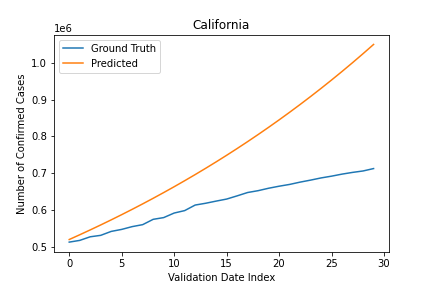
\includegraphics[width=\linewidth]{./figures/Section2_AR_Cali_Conf.png}
  \caption{Confirmed Cases in California predicted using AR}
\end{figure} 
Our final round 1 MAPE using AR was $4.12$
The issue with our implementation of the model is that we did not enforce the stationarity of the data which 
is a prerequisite for the model. A stationary time series is one whose properties do not depend on the time at 
which the series is observed \cite{forecasting}.
This therefore shows AR's difficulty in accounting for the trend since stationary
data is devoid of one. Therefore we needed a model that was able to account for data with a trend. This is why we chose to 
explore the Autoregressive Integrated Moving Average (ARIMA) model. The Moving Average (MA) portion of ARIMA states that 
future time steps are predicted as a linear combination of previous forecast errors. The equation for this model is \cite{forecasting},
\begin{equation}
y_t = c + \sum_{i=1}^{q} \theta_i \epsilon_{t-i}
\end{equation} 
Where $\theta_i$ are the learned weights, $c$ is the bias term and $\epsilon_i$ are the white noise error terms that are 
seen in equation 1. Since we look at the last $q$ time steps, this is known as a MA(q) model.
Hence, a combination of the AR model and the MA model will reduce the compounding error problem from before since we
take the forecast errors into account. However both AR and MA models require data to be stationary which as shown before is not
the case. A way to make data stationary is by looking at the difference of contiguous time series values $y'_t = y_t - y_{t-1}$
as opposed to the values themselves. This process of differencing can be done multiple times if the initial differencing does
not yield a stationary time series.

Therefore, the ARIMA model incorporates differencing to give the forecasting equation \cite{forecasting},
\begin{equation}
  y'_t = c + \sum_{i = 1}^{p} \phi_i y'_{t-i} + \sum_{j=1}^{q} \theta_j \epsilon_{t-j} + \epsilon_t
\end{equation}
Which we see is a combination of equations 1 and 2 but on differenced values. Thus the $\epsilon_j$ are white noise errors for
$y'_j$ not the original time series $y_j$. As we mentioned, differencing can occur many times until stationarity is enforced,
we let the the number of time the data is differenced be denoted as $d$ the degree of differencing. Furthermore, we are
already aware of the parameters $p$ and $q$ from the respective AR and MA models. Hence we denote the above equation as an
ARIMA(p,d,q) model. 

To implement this model, we used the ARIMA module from the statsmodels package \cite{statsmodels}. There are, however, many
ways to find the optimal $p,d,q$ values. Initially we thought that since our metric of evaluation is MAPE, we could optimize
these parameters with respect to a validation MAPE and use those parameters to predict the future cases and deaths for a 
particular state. To do this, a simple grid search was done where $p,d,q$ values ranged from $1$ to $10$ and the tuple with the
lowest validation MAPE for that state was chosen. Initially we chose a validation size of 30 days. This yielded a final round 1 MAPE of $3.44$.
Although this was better than the AR model, it was still below the baseline MAPE. In addition, we saw an increased number 
of stationarity and convergence errors with our optimized set of tuples for certain states. In these cases, we had to resort to
using our naive AR implementation as backup. This indicated that our tuple was not fully capturing the trends in our data
by being optimizing for 30 days prior. 

Hence we chose to reduce our validation size to 7 days instead to see if having a larger amount of data and using a more
recent validation set would lead to a more representative optimal $p,d,q$ tuple. This was indeed the case as we were able to
get a round 1 MAPE of 2.96. We still ran into the stationarity and convergence errors and did have to use AR as a backup.
In this vein, we reduced the validaiton size further to only 3 days but this led to a MAPE of 4.71 indicating that we overfit
our validation data. 

The auto arima module from the pmdarima package \cite{pmdarima} uses a grid search similar to before to find the optimal
tuple. However, auto arima uses statistically rigorous stationarity tests (such as Augmented Dickey Fuller) to find 
the optimal order of differencing $d$ after which the optimal $p,q$ are found by minimizing the Akaike Information Criterion (AIC).
AIC is a measure of the quality of a model, it measures the likelihood of a model to predict future values \cite{AIC}. The equation
to calculate AIC is given by \cite{AIC},
\begin{equation}
  AIC  = -2 \cdot \ln(L) + 2k
\end{equation} 
Where $L$ is the likelihood of the model, and $k$ is the number of estimated parameters. A model with a lower AIC value
indicates a model of better quality. Optimizing on by MAPE on a validation set runs the risk of being overfit to the validation
set as seen when we reduced our validation size to 3 days. Hence when looking a generalizable models for our round 2 submission,
it was important that we did not overfit to our current data. By using a measure that is trained insample and does not depend
on a validation set, the generalizability of the model increases. By optimzing for AIC we did get a lower MAPE than our previous
models so this was chosen as the optimization criteria when a state is trained using this method.


\subsection{HOLT}
\subsection{Conclusions}

While the HOLT model typically gives us the lowest overall MAPE, it
consistently underperforms on certain states. Linear Regression and ARIMA may
yield significantly better results for these "problem states". However, it is
not always easy to tell which states are going to cause problems with the HOLT
model -- performance varies significantly based on the shape of the latest
batch of test data. This heterogeneity makes it very difficult to pick a
"favored model" for our time series predictions. 

Not all of our results were mixed. While model performance varied significantly
based on the target state, the "optimal hyperparameters" used to train these
models do not change significantly on a state-by-state basis. By performing
grid search on each model's hyperparameters, we developed a group of
parameterized models that handle general state data reasonably well. 


\section{Model Design}

The pros and cons (as well as the relative efficacy) of each model have already
been discussed. Faced with such a diversity of model performance, we opted to
use a hybrid model for our overall submission. Rather than cherry picking the
best-performing models for each state, we opted to use an automated approach. 

Suppose we have to predict $m$ days into the future. 

Our model first segregates the data by state. For each state,

\section{TODO TODO TODO TODO}
% did I mention this is TODO?

First, we segregate the data. Given $n$ days of training data, our model uses
the first $n-2$ days to train on (we'll call this set $T$) and the last $2$
days as a validation dataset (we'll call this subdivision $V$). 
We then train Linear Regression, HOLT, and ARIMA models on $T$, predicting
$m+2$ days into the future. We take the first $2$ days of these predictions,
and calculate the MAPE using $V$. After comparing the MAPEs of each model on
$V$, we choose the model that gives us the lowest MAPE for that particular
state, and return the remaining $m$ days of predictions. 

After observing our hybrid model, we noted two trends: 
\begin{itemize}
\item 
Splitting our data into $T$ and $V$ caused some of our models to
underperform. This is because they effectively had to predict $m+2$ days into
the future as opposed to $m$ days (the first two days, of course, were used for
our validation and model selection). This underperformance wasn't uniform;
HOLT tended to give us relatively accurate predictions, while linear regression
tended to underpredict the number of deaths. 
\item
Different models often give similar MAPEs when evaluated on $V$. 
\end{itemize}

Given these two points, we added an $\epsilon$ "margin" term to our final
implementation. If two models perform comparatively (ie. within $\epsilon$ MAPE
of each other) on $V$, then our framework prefers the model that "generalizes
better" as per our heuristic observations. For example, if linear regression
and HOLT both get an MAPE of $8.675309 \pm (\epsilon = 0.001)$, our framework
will use HOLT to predict the values for the state. Our framework prefers HOLT
to linear regression if the MAPEs are similar, but doesn't put ARIMA into this
"margin" framework (ie. if ARIMA yields the lowest MAPE, ARIMA will always be
chosen). 

\bibliographystyle{ACM-Reference-Format}
\bibliography{report}

\end{document}
\endinput
